\documentclass[12pt]{article}

\usepackage{sbc-template}
\usepackage{graphicx,url}
\usepackage[latin1]{inputenc}  

\usepackage{../Utils}
\usepackage{implementation}     
\sloppy

\title{Beyond ASCII, parsing programs with graphical presentations \\{\small \version}}

\author{Martijn M. Schrage\inst{1}}


\address{Institute of Information and Computing Sciences\\ Utrecht University\\
    Utrecht, The Netherlands
  \email{martijn@cs.uu.nl}
}

\begin{document} 

\maketitle

\begin{abstract}
% 15 lines
Proxima is generic editor. although it has wp facilities, graphs, very suitable for programming languages. Structural and presentation-edit.

Pres may be graphical: fraction. When edited, need to parse this.

Solution that uses combinator parsers for simple stuff. Also automatic whitespace handling
\end{abstract}
     
\bc

Introduction (2)

Proxima's layered architecture (2)
- explanantion of presentation/interpretation processes
- overview of levels and layers
  (much can be taken from thesis chapter)
  
Presentation process
  
  Xprez (2)
  - short version of thesis chapter
  Presentation (2)
  - explanation of AG system
  - structural vs parsing
  - examples
   
Interpretation process 
  Scanner (2)
  - regular expression for specifying tokens
  - example
 
  Parser  (2)
   - structural vs parsing
   - uuag parser with only a few extra things
   - example
  Error handling in parser and scanner
 
Related work (1/2)
- synthesizer generator
- eclipse
- barista

Conclusions (1/2)

\ec

\section{Introduction}

\bl
\o what is Proxima~\cite{schrage04Proxima}.
\o Generic editor for variety of documents, but very suitable for editors programming language.
\o modeless combination of structure editing and free editing in the presentation
\o nothing is primitive, hence very customizable
\o example applications
\o Editor for Baysian networks
\o Generic editor as IDE
\o by giving type, pres, and parser, we get an environment almost for free
\o Helium editor
\o Implementation of Proxima
\o overview of paper 
\el
\bl
\o contribution: algorithm for parsing mix of graphical and textual presentations.

\el

\bc
\begin{figure}[ht]
\centering
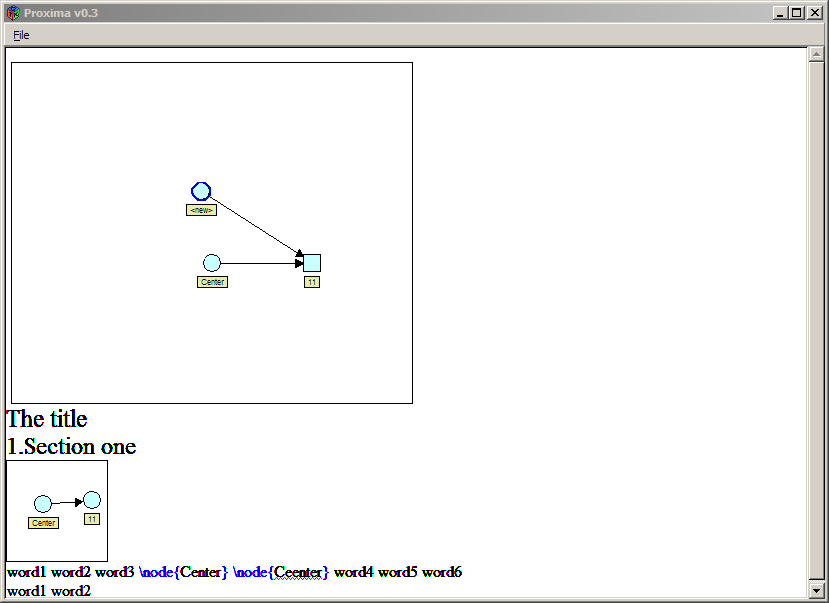
\includegraphics[width=\textwidth]{images/screenshots/BayesDocEditor}
\caption{The Bayesian network documentation editor}
\label{fig:bayesEditor}
\end{figure}
\ec

%%%%%%%%%%%%%%%%%%%%%%%%%%%%%%%%%%%%%%%%%%%%%%%%%%%%
%
\section{Proxima's layered architecture} \label{sec:architecture}
%
%%%%%%%%%%%%%%%%%%%%%%%%%%%%%%%%%%%%%%%%%%%%%%%%%%%%

The core architecture of Proxima consists of a number of layers, which only communicate with their direct neighbors. This layered structure is based on the staged nature of the presentation process. Instead of mapping a document directly onto its final rendering, it is first mapped onto an intermediate data structure. This intermediate data structure is mapped onto another intermediate data structure, until the last intermediate data structure is mapped onto the rendering.

..  the positions at which the document, the rendering, and the intermediate data structures reside are called {\em data levels}. Between each pair of levels is a {\em layer}, which is a component that maintains the mappings between the levels. Figure~\ref{fig:levelsAndLayers} schematically shows the levels and layers of Proxima. Only two data levels are visible to each layer: a higher and a lower level.

\begin{figure}[ht]
\centering
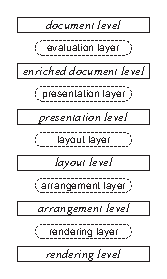
\includegraphics[width=4cm]{images/LevelLayerNames}
\caption{The levels and Layers of Proxima.}
\label{fig:levelsAndLayers}
\end{figure}

A data level in Proxima is not just an intermediate value in the presentation computation, but an entity in its own right. Together, the data levels constitute the state of the editor. The six data levels of Proxima are:


\begin{description}
\item[Document:] The edited document, the type of which is specified by a DTD or an EBNF grammar.

\item[Enriched Document:] The document enriched with computed information.

\item[Presentation:] A logical description of the presentation of the document, consisting of rows and columns of presentation elements with attributes. The presentation also supports formatting based on available space (e.g.\ line/page breaking).

\item[Layout:]  Presentation with explicit whitespace.

\item[Arrangement:] Formatted presentation with absolute size and position information.

\item[Rendering:] A collection of user interface commands for drawing the absolutely positioned and sized arrangement.
\end{description}



\bl
\o explain why layered
\o briefly explain both components of each layer
\o Editing takes place either at the document, or at the layout level.
\o mapping from doc to ren
\o explain layers may be skipped skipping of layers
\o implementation: layer combinators.
\o sometimes awkward, because we have to conform to the layers.
\o but this has advantages: new GUI lib in a matter of days.
\el

\bl
\o Presentation sheet
\o Parsing sheet
\o Scanner sheet
\o (evaluation/reduction sheets)
\el
In this paper, we focus mainly on the presentation layer and layout layer, and more specifically on the scanner and parser in these layers.


%%%%%%%%%%%%%%%%%%%%%%%%%%%%%%%%%%%%%%%%%%%%%%%%%%%%
%
\section{The document structure}
%
%%%%%%%%%%%%%%%%%%%%%%%%%%%%%%%%%%%%%%%%%%%%%%%%%%%%

\bl
\o Document is main data type
\o Haskell types, no parameters
\o fields to store token id's for handling whitespace and focus
\o holes and parse errors added to each nonterminal
\o holes are for structure editing.
\el

\begin{verbatim}
data Exp = DivExp exp1:Exp exp2:Exp                      { idP0:IDP }
         | IfExp exp1:Exp exp2:Exp exp3:Exp              { idP0:IDP idP1:IDP idP2:IDP }
\end{verbatim}

\section{The presentation process}

Before discussing the scanner and parser components, we briefly discuss the presentation process. Presentation component, there is a specification (presentation rules) that map the document (more precisely the enriched document) to presentation target language, which is a Haskell combinator language Xprez. The rules are an attribute grammar.

%%%%%%%%%%%%%%%%%%%%%%%%%%%%%%%%%%%%%%%%%%%%%%%%%%%%
%
\subsection{The {\Xprez} presentation language} \label{sect:xprez}
%
%%%%%%%%%%%%%%%%%%%%%%%%%%%%%%%%%%%%%%%%%%%%%%%%%%%%

\Xprez is a combinator library for specifying graphical presentations with support for stretching and alignment. For this paper, a short overview of the language suffices. A more complete description can be found in~\cite{schrage04Proxima}.

The basic building blocks of \Xprez are strings, tokens and graphical elements such as lines, circles, or images. 



\bl
\o basic \p{text} 
\o mention a \p{token}
\o composite \p{row}, \p{col}, \p{overlay}
\o alignment.
\o modification of attributes: with
\o also popup menus.
\o locators that denote path and node of a presentation tree.
\el

An Xprez example:

\begin{footnotesize}
\begin{verbatim}
pad xp = row [ hSpace 2, xp, hSpace 2 ]
shrink e = e `withFontSize_` (\fs -> (70 `percent` fs) `max` 10)
frac e1 e2 = let numerator   = hAlignCenter (pad (shrink e1) )
                 denominator = hAlignCenter (pad (shrink e2) )
             in  colR 2 [ numerator, vSpace 2, hLine
                        , vSpace 2, denominator ] `withHStretch` False
\end{verbatim}
\end{footnotesize}

The non-primitive library function \p{hAlignCenter} centers its argument horizontally.


\bc
%																
\subsection{{\Xprez} presentation model}

Similar to the document formatting languages \TeX ~and Lout~\cite{kingston93lout}, {\Xprez} is a box language with support for flow layout. A presentation is a value of the abstract type \p{Xprez}, and is either an atomic box containing a text or a graphical object, or a composite box that contains a list of child presentation boxes.  We construct \p{Xprez} values in the functional language Haskell, using a number of primitive functions that are described in Section~\ref{sect:primitives}.


A presentation tree in {Xprez} represents an attribute grammar with inherited and synthesized attributes. Presentation attributes that are typically specified for an entire subpresentation, such as color and font size, are inherited attributes.  \b\c (going downward in the tree)\e\c On the other hand, presentation attributes that are set by a child and used by its parent, such as  reference lines and size information, are synthesized attributes. Figure~\ref{xprezattributes} shows the two Haskell records  \p{Inh} and \p{Syn} that are used to model the inherited and synthesized presentation attributes. The figure also shows the type of each attribute. 

The \p{hRef} and \p{vRef} attributes specify the reference lines that are used for aligning boxes horizontally and vertically when combined in composite presentations. Note that the vertical-reference line is in fact a horizontal line and vice versa. The term vertical-reference line stems from the fact that it is used for vertical alignment; modifying the vertical-reference line affects the vertical position of the presentation. 

The boolean attributes \p{hStretch} and \p{vStretch} specify whether or not the presentation is allowed to stretch in horizontal or vertical direction. The remaining attributes are self-explanatory: \p{fontFamily}, \p{fontSize}, \p{textColor}, \p{lineColor}, \p{fillColor}, and \p{bgColor}. In the future, this set will be extended with other attributes such as line and font style, and attributes for modeling edit behavior (e.g.\ \p{onMouseClick~::~EditCommand}).
 
\b\c
The presentation tree is transformed into an attribute grammar in which the font, style, and color properties are inherited attributes that go down in the tree, and alignment and stretch properties are synthesized attributes that go up in the tree. In the Haskell types, this division is visible in the fact that the properties are modeled using two records: \p{Inh} for inherited properties, and \p{Syn} for synthesized properties.
\e\c

%																
\subsection{{\Xprez} primitives} \label{sect:primitives}

The first five combinators in Figure~\ref{xprezprim} specify atomic presentations. The \p{empty} combinator has a presentation that is invisible and takes up no space; it is the neutral element for various presentation compositions. A string is presented with combinator \p{text}, and a rectangle with combinator \p{rect}. The \p{poly} combinator takes a list of relative coordinates between (0.0, 0.0) and (1.0, 1.0) and produces a line figure that connects these points. The coordinates are relative because the final coordinates depend on the size of the \p{poly} presentation. Finally, \p{img} can be used to display external images. The argument is a string that contains the path to the image file. In a future version, an \p{img} term may also contain a reference to an image that is encoded as part of the document.

Except for \p{text}, the reference lines of an atomic presentation both have coordinate 0 (i.e.\ the north-west corner). For \p{text},  the vertical-reference line is the baseline of the text and the horizontal-reference line is at 0. By default, a  simple presentation does not stretch.

\begin{figure}
\begin{footnotesize}
\begin{center}
\begin{footnotesize}
\begin{verbatim}
empty             :: Xprez
text              :: String -> Xprez             
rect              :: Xprez                       
img               :: String -> Xprez             
poly              :: [ (Float, Float) ] -> Xprez 
row, col, overlay :: [ Xprez ] -> Xprez          
rowR, colR        :: Int -> [ Xprez ] -> Xprez   
matrix            :: [[ Xprez ]] -> Xprez
format            :: [ Xprez ] -> Xprez
\end{verbatim}
\end{footnotesize}
\caption{The {\Xprez} primitives} \label{xprezprim} 
\end{center}
\end{footnotesize}
\end{figure}

The remaining primitives in Figure~\ref{xprezprim} specify composite presentations. The behavior of columns (\p{col}) is equal to that of rows (\p{row}) with the horizontal and vertical directions swapped. Hence, we only discuss the \p{row} primitive. In a row, each child presentation is placed immediately to the right of its predecessor, with their vertical-reference lines aligned. Horizontal-reference lines have no effect on the positioning in a row.

\begin{center}
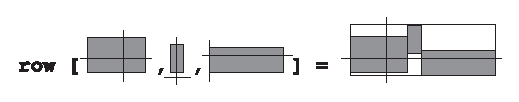
\includegraphics[width=3.2in]{images/row}
\end{center}

The bounding box of a row is the smallest rectangle that encloses all elements of the row. The vertical-reference line of the row is equal to the aligned reference lines of the children, whereas the horizontal-reference line is taken from the first child. In order to use the horizontal-reference line from one of the other children, we can use the \p{rowR} combinator. The integer argument of \p{rowR} specifies which child determines the horizontal-reference line for the row, with 0 denoting the first child. 

By default, a row stretches in horizontal direction if one of its children does, and it stretches in vertical direction if all children stretch vertically. The defaults may be overridden by setting the stretch attributes with the method that is  shown in the next section. 


Because \p{row}, \p{column} and \p{matrix} do not allow their children to overlap, we need a special combinator for overlapping presentations. The \p{overlay} combinator places its children in front of each other, while aligning both the horizontal and vertical-reference lines. It can be used to create underlined text, for example. Because alignment takes place on both reference lines and hence all child reference lines overlap, no special \p{overlayR} combinator is needed.

A flow layout can be achieved with the \p{format} combinator for paragraph formatting. The combinator takes a list of presentations as argument and splits this list into rows based on the available horizontal space. The resulting rows are placed in a column.  Because \p{Xprez} does not yet have a page model, only horizontal formatting is supported. 
\ec

\subsection{Document presentation}

For the presentation of the document, as well as for the computation of derived values and structures, Proxima uses the attribute grammar formalism (or AG). The presentation sheet is file with an AG definition, which is compiled to a Haskell program by the Utrecht University AG compiler~\cite{swierstra08ag}.

For each non-terminal, the AG defines a synthesized attribute \p{pres} of type \p{Presentation}.\todo{params} In the rule for \p{pres}, the presentations of child fields can be used. Besides the presentation, arbitrary synthesized and inherited attributes can be defined on the document tree. This way it is easy to specify static checks or for example the computation of all variables in scope at a certain document location. Moreover, external Haskell modules can be called, allowing for complex computations, such as type checking.

% also possible edit operations specific to the nonterminal.

A presentation may be either {\em structural} or {\em parsing}, with the difference that parsing presentations may be edited at the presentation level whereas structural presentation may not (although they may have parsing descendents that will be editable). 

A parsing presentation consists of a sequence of tokens, which may be strings or structural presentations. It is provided with a parser that is applied to the sequence of tokens when it has been edited. \todo{only top level if it is an immediate child of a structural}
\bl % or maybe near example
\o row is now used for making token sequence tokens.
\o we can enforce that only \p{token}s appear with a GADT!
\el


Since a structural presentation may not be edited at the pres,  be edited at the presentation level.
On the other hand, a parsing presentation consists of tokens (either strings or structural presentations) and is provided with a parser in the presentation sheet. Parsing presentations may be edited at the presentation level, after which the parser is applied to obtain the updated subtree.


\begin{footnotesize}
\begin{verbatim}
SEM Exp
  | IfExp loc.pres = parsing $ row  $ [ key @idP0 "if",   @exp1.pres
                                      , key @idP1 "then", @exp2.pres
                                      , key @idP2 "else", @exp3.pres ]
  | DivExp
      loc.pres = structuralID @idP0 $ frac @exp1.pres @exp2.pres
                  
key str = token str `withColor` blue 
\end{verbatim}%$
\end{footnotesize} % put this in a figure?

\bl
\o add structural example without id
\el

\p{frac} is the function defined in Section~\ref{sect:xprez}

In each presentation rule there need to be a number of default function applications, for example to handle the display of focus, and to mark the document location in the presentation tree. Such functions may be applied by the writer of the presentation sheet, but this is awkward and error prone. Hence, rather than the definitions of synthesized attributes \p{pres} for each nonterminal, the presentation sheet contains definitions of a local attribute \p{pres}. An automatically generated rule for the synthesized \p{pres} then uses the local \p{pres} and adds the default functionality to it.

\subsection{Document layout}

The layouter is currently not parameterized by any sheet
\bl
\o it adds layout explicitly, by looking it up in the map, and also restores the focus
\o if focus restore fails, focus is set on old coordinates (usually okay, explain when not)
\el


%%%%%%%%%%%%%%%%%%%%%%%%%%%%%%%%%%%%%%%%%%%%%%%%%%%%
%
\section{Scanner}
%
%%%%%%%%%%%%%%%%%%%%%%%%%%%%%%%%%%%%%%%%%%%%%%%%%%%%

The basic function of the scanner is to map strings containing characters to tokens, which are specified by the user in the scanner sheet. But in Proxima, the scanner also performs several other functions. Any structural presentations that appear in the stream of tokens are put in special tokens. Such structural presentations may contain other structural presentations, or again parsing presentations, which are recursively scanned. Apart from this scanner also handles graph presentations. 


\bl
\o result is Structural [.. [PresentationTk]..]
\el

\subsection{The \p{Token} type}

Figure~\ref{fig:tokenType} shows a simplified version of the \p{Token} data type. A number of type parameters that are not important for this discussion are hidden, as well as the constructors that have to do with Proxima's support for graph presentations. 
\begin{figure}
\begin{center}
\begin{tabbedCode}
data Token Location userToken\\ 
~~\= =  StructuralTk \= Position \= IDP Location Presentation \\
  \>                \> [Token node userToken]\\
  \> | ParsingTk    \>          \> IDP Location (Parser userToken)\\
  \>                \> [Token node userToken]\\
  \> | UserTk       \> Position IDP Location userToken String \\
  \> | ErrorTk      \> Position IDP String \\
\end{tabbedCode}
\caption{The \p{Token} data type} \label{xprezprim} 
\end{center}
\end{figure}

All constructors have an \p{IDP} field. used to associate the token with whitespace/focus. The \p{Position} only for elts that are actually parsed, not for \p{ParsingTk}.\todo{maybe idp also not necessary}.  \p{Maybe node} is document location
The \p{Location} field refers to the node in the document tree from which the token originated. It is used when parsing structural presentations.\todo{ref to section?}

The last constructor \p{ErrorTk}, is used to represent lexical errors. It's use is explained in Section~\ref{sect:parseScanErrors}

\bl
\o parsing has a parser associated
\o location in usertoken is for reuse (talk about this here?)
\o location in structural and parsing is for auto structurals
\o for structurals also for restoring fields that are note presented
\o lists of tokens are children.
\el

% Not shown: Presentation in StructuralTk

\subsection{The scanner sheet}

The lexical analysis of textual tokens is based on the Haskell lexical analyser generator Alex~\cite{marlow07alex}. Alex is a tool that generates an efficient lexical analyser based on a description of the tokens to be recognized in the form of regular expressions. It is comparable to the lex and flex tools for C and C++.

An editor designer has to define the data type \p{UserToken} and provide an Alex specification that defines the tokens. Figure~\ref{fig:scannerSheet} shows an example \p{UserToken} and scanner sheet. The Alex specification consists of a a number of macro definitions followed by a set of rules, each defining a token. A rule is a regular expression together with an action that constructs the token.

\begin{figure}
\begin{center}
\begin{footnotesize}
\begin{verbatim}
data UserToken = Ident String | Op String | Int Int

$lower = [a-z]
$upper = [A-Z]
$alpha = [$lower $upper]
$digit = 0-9		
$symChar = [\+ \- \= ]
tokens :-
 $digit+                       { mkToken $ \s -> Int (read s) }
 $symChar+                     { mkToken $ \s -> Sym s }
 $lower [$alpha $digit \_ \']* { mkToken $ \s -> Ident s }
\end{verbatim} %$
\end{footnotesize}
\caption{Example \p{UserToken} and scanner sheet} \label{fig:scannerSheet} 
\end{center}
\end{figure}

The only difference between a normal Alex description and a Proxima scanner sheet is that each action needs to be preceded by a \p{mkToken} application. The \p{mkToken} application takes care of passing the internal scanner state, and constructs a \p{UserTk} alternative of type \p{Token}. \todo{mention it assigns IDP}



\subsection{Scanning the presentation}

Scanner based on structural/parser

% How the tokenizer works:
\head{Structural presentation}

A structural presentation of a document node is an Xprez tree that may contain presentations of child nodes. The scanner traverses the presentation tree and makes a recursive call on each child presentation that is encountered. It also stores the presentation in case of a parse error (recursively scanned). Yielding a StructuralTk.

\head{Parsing presentation}

A parsing presentation only consists of a column of rows, which contain either strings or structural presentations. scanner creates sequences of characters . Structurals are put in Structural tokens. the sequences of characters are converted to tokens by applying the Alex scanner.


\subsection{Handling whitespace}

% Whitespace
In order to use the automatic whitespace recognition, the following rule must be added to scanner sheet:

\begin{footnotesize}
\begin{verbatim}
  [\n \ ]+        { collectWhitespace }
\end{verbatim} %$
\end{footnotesize}

The result is that the scanner will also put whitespace tokens in the result of the If enabled, the final list of tokens will contain whitespace tokens. These are associated with the id of the preceding token's (may be structural).

% first token whitespace

\subsection{An example}

To clarify the previous discussion, we give an example of a scanned presentation. So this partially graphically presented function:
\begin{center}
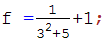
\includegraphics[width=1in]{images/fraction}
\end{center}
\todo{add some whitespace}

leads to the following tokens:\todo{maybe add locators and paths}
\begin{tabbedCode}
ParsingTk \= \\
~~ \= [ UserTk$_0$ (Ident "f") \\
      \> , UserTk$_1$ (Op "=") \\
      \> , StructuralTk$_2$ (DivExp (IntExp 1) (PlusExp ...))\\
      \> ~~ ~~ \= [ ParsingTk [ UserTk$_3$ (Int 1)] \\
      \>            \>  , ParsingTk  \= [ StructParsingTk$_4$ (PowerExp (IntExp 3) (IntExp 2))\\
      \>            \>                 \> ~~~~ \= [ ParsingTk [ UserTk$_5$ (Int 3) ] \\
      \>            \>                 \>           \>  , ParsingTk [ UserTk$_6$ (Int 2) ] \\
      \>            \>                 \>           \> ] \\
      \>            \>                 \> , UserTk$_7$ (Op "+") \\
      \>            \>                 \> , UserTk$_8$ (Int 5) \\
      \>            \>                 \> ] \\
      \>            \> ] \\
      \> , UserTk$_9$ (Op "+") \\
      \> , UserTk$_{10}$ (Int 1) \\
      \> ] \\
\end{tabbedCode}

maybe: explain that all tokens in a parsingTk contain refs to their originating nonterminal in the document. In case of incomplete presentation, we reuse the fields from that node. Fragile. Copy/paste, retyping, it may get lost. So only for non-essential things. 

and a map containing the whitespace (and focus)

\begin{tabbedCode}
Whitespace = [ 0 -> (0,1), 1-> (0,1), 1 -> (1,0) ]
\end{tabbedCode}

Also put document node and path




%%%%%%%%%%%%%%%%%%%%%%%%%%%%%%%%%%%%%%%%%%%%%%%%%%%%
%
\section{Parsing}
%
%%%%%%%%%%%%%%%%%%%%%%%%%%%%%%%%%%%%%%%%%%%%%%%%%%%%

Unlike normal parsers, which take a list of tokens to produce a value, the Proxima parser is a function that takes only one token as input. This token can be either a structural token or a parsing token. In case of a structural token, the value is constructed automatically from the list of child tokens. If the token is a parsing token, its list of children is fed into the parser that was specified in the presentation sheet.

\subsection{Structural presentations}

A structural token corresponds to the presentation of a certain document node and contains a list of tokens that correspond to child-presentations that were part of the presentation of that document node. Each child may be presented multiple times, or even not at all. Furthermore, the order in which the child presentations appear may not correspond to the order of the children in their parent node.

Maybe an example? 
Nevertheless, we can parse a structural token automatically, since all tokens contain a \p{Locator} reference to the document node from which they were presented. \todo{Not destroyed because structurals not edited.}  By calling the parser recursively on the list of tokens, we obtain the document nodes for each child. .. The child tokens (either structural or parsing) contain document locators from which we can derive the child number.


Each token has ref to parent/path (cannot be broken in structural)

recognizeStructural
has a list of tokens, either structural or parsing. Each has information on origin as a path. so group them with their index in the parent.

Now recursively recognize each child. Either structural (this function), or Parsing (section ..). 

For any children that were not part of the presentation, we take the previous value from the locator of the StructuralTk that is currently parsed. And for doubles, at the moment, we take the first. But as soon as we keep track of dirty bits in the presentation, we take the edited child. If more edited either signal error, or take one. This can be prohibited by enforcing a parse cycle if we start editing another child.

\todo{untyped, but safe}

\subsection{Parsing presentations}

A \p{ParsingTk} token contains a parser that returns a value of .  a  we 
\bl
\o convert list of \p{Token} to document structure.
\o combinator parser with error recovery~\cite{swierstra03polishParsers, swierstra08parserCombinators}
\o because of extra state (hidden presentations), and presentation ids, little bit extra info is kept
\o only when needed
\o mention that holes need to be explicitly parsed?
\o in fact other module that parses tokens to document nodes can be used. Parsec~\cite{leijen08parsec}
\o Example
\el

\section{Parse errors} \label{sect:parseScanErrors}

On a parse error, we don't get a tree, so tricky to present. Parse and present should be identity (with squiggly for error). Won't appear in structural presentations, unless something is wrong in the presentation. In this case error is signaled. Problem for editor builder. In parsing presentations. Parse errors are normal, during programming most of the time not syntactically correct.

Approach: all nonterminals have a parseErr constructor. Insteafd of a value of type T, we get ParseErr\_T (is a value of type T). The parse error alternative has error loc + message and a list of tokens.

On presentation, the tokens are presented, and the location of the error gets a squiggly. Whitespace is added by the layouter as for any other token. Message is available as an attribute.

% lexical errors
Lexical errors pose a problem, since Alex stops at the character of the lexical error. Hence any following whitespace is not recorded. However, we do want the presentation of the lexical error to stay the same. Hence, an error token \todo{annoying that we haven't explained parse errors yet} is treated specially and expands its whitespace into spaces and line breaks.


%%%%%%%%%%%%%%%%%%%%%%%%%%%%%%%%%%%%%%%%%%%%%%%%%%%%
%
\section{Related work}
%
%%%%%%%%%%%%%%%%%%%%%%%%%%%%%%%%%%%%%%%%%%%%%%%%%%%%

\todo{more?}

\head{Eclipse}

Eclipse~\cite{eclipse2001} is a Java-based platform for building integrated development environments. The platform has an open architecture, and can be easily extended through a plug-in mechanism. Eclipse includes a syntax-recognizing Java editor, which supports in-place type information, refactoring, as well as document-oriented edit operations. 

Though it is not exactly a generic editor, Eclipse does have facilities for creating syntax-recognizing source editors. Unfortunately, building a code editor similar to the Java editor for a different language, requires a substantial amount of programming. Moreover, the presentation of the code is rather limited (lines of text), and there is no support for derived values appearing in the presentation.

\head{Barista, Citrus}

Barista~\cite{KoMyers06Barista} is a powerful framework for building code editors. It is built on top of Citrus~\cite{KoMyers05Citrus}, which is a UI toolkit together with an object-oriented language. Although Barista is targeted at code editors, the presentation of the code can be visual, for example allowing for images to appear in comments, or having graphical presentations of code. The editors created with Barista are syntax directed, but presentation-oriented editing is available. 

Because of the orientation towards code editing, word-processing editors will be harder to specify in Barista. The same holds for editors for which the structure of the presentation does not follow the structure of the document. Barista has no special support for derived values in the presentation or for editable derived structures.



%%%%%%%%%%%%%%%%%%%%%%%%%%%%%%%%%%%%%%%%%%%%%%%%%%%%
%
\section{Conclusion} 
%
%%%%%%%%%%%%%%%%%%%%%%%%%%%%%%%%%%%%%%%%%%%%%%%%%%%%

\bl
\o more static checks are possible
\o easy ways to increase speed after change management
\o dtd pres and parser give simple environment
\o use ag to add static/type checks
\el

%%%%%%%%%%%%%%%%%%%%%%%%%%%%%%%%%%%%%%%%%%%%%%%%%%%%
%
% References

\bibliographystyle{sbc}
\bibliography{../proxima}

\end{document}
